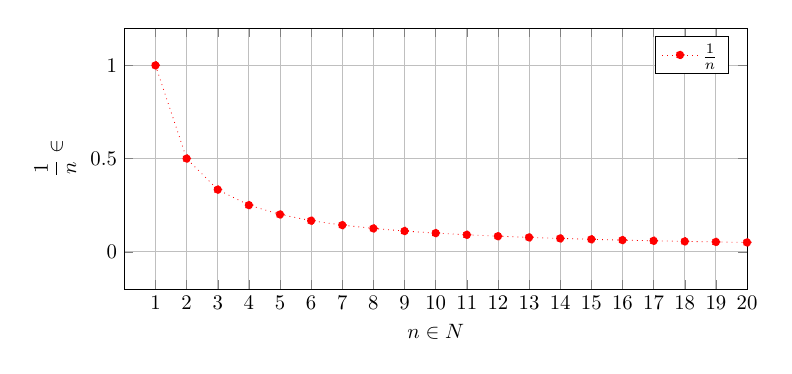
\begin{tikzpicture}[scale=.75]
	\begin{axis}[
		xlabel={$n \in \mathbb{N}$},
		ylabel={$\displaystyle\frac{1}{n}\in\R$},
		ymin=-.2, ymax=1.2,
		xmin=0, xmax=20,
		xtick={1,2,...,20},
		ytick={0,0.5,1},
		grid=major,
		width=\textwidth,
		height=6cm,
		domain=1:20,
		samples=20,
		legend pos=north east
		]
		% Plot points for 1 - 1/n
		%		\addplot[line width=.25mm, only marks, red, mark=x] plot (\x, 1 - 1/\x);
		\addplot[red, mark=*, dotted, mark options={fill=red}] plot (\x, 1/\x);
		\addlegendentry{$\frac{1}{n}$};
		
		% Draw horizontal line showing upper bound (y=1)
%		\addplot[dashed, magenta, line width=.5mm] coordinates {(0,1) (30,1)};
%		\node[magenta] at (axis cs: 3,1.1) {Upper Bound $1$};
		
		% Draw horizontal line showing lower bound (y=0)
%		\addplot[dashed, cyan, line width=.5mm] coordinates {(0,0) (30,0)};
%		\node[cyan] at (axis cs: 3,-0.1) {Lower Bound $0$};	
	\end{axis}
\end{tikzpicture}